\documentclass[
  10pt,
  a4paper,
  oneside,
  headers,
  headinclude,
  footinclude,
  BCOR5mm,
]{article}
\usepackage{ragged2e}
\usepackage{graphicx}
\usepackage{subcaption}
\usepackage{beramono}
\usepackage[utf8]{inputenc}

\graphicspath{ {./images/} }

\title{IT Projekt}
\date{06.05.2019}
\author{Ivaylo Lenkov Ivanov}

\begin{document}

\begin{titlepage}
  \maketitle
  \tableofcontents
  \pagebreak
  \listoffigures
\end{titlepage}

\justify
\section{Einführung}
Für ein Hauptziel hat dieses Projekt eine virtuelle Umgebung zu bilden und in dieser Umwelt die grundlegende Physik zu simulieren. Die virtuelle Welt ähnelt ein Computerspiel.

\begin{figure}[h]
  \centering
  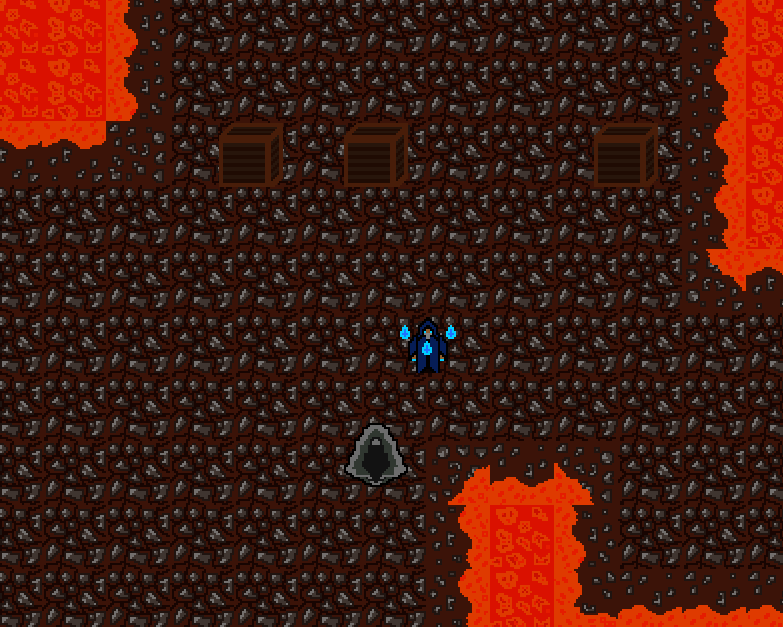
\includegraphics[scale=0.25]{VirtualEnvironment}
  \caption{Die virtuelle Umgebung}
  \label{fig:Umgebung}
\end{figure}

\justify
Der Benutzer steuert eine virtuelle Figur.

\begin{figure}[h]
  \captionsetup{justification=raggedright,singlelinecheck=false}
  
\includegraphics[scale=0.10]{MageCharacter}
  \caption{Avatar}
  \label{fig:Avatar}
\end{figure}

\justify
Der Avatar kann sich in dem Terrain bewegen und Eiszapfen in jeden Richtung feuern. Die Anfangsszene dem Spiel hat vier Spielobjekte --- drei Kasten und ein Stein.

\begin{figure}[h]
  \begin{subfigure}{0.5\textwidth}
    
\includegraphics[width=0.3\linewidth, height=2cm]{Box}
    \caption{Kasten}
    \label{fig:Kasten}
  \end{subfigure}
  \begin{subfigure}{0.5\textwidth}
    
\includegraphics[width=0.3\linewidth, height=2cm]{Stone}
    \caption{Stein}
    \label{fig:Stein}
  \end{subfigure}

  \caption{Spielobjekte}
  \label{fig:Spielobjekte}
\end{figure}

\justify
Mit den Kisten kann der Anwender interagieren. Das heißt, dass der Benutzer sie herumschubsen kann und auch auf sie Eiszapfen zu schießen. Das kann zu der Zerstörung diesen Kästen führen. Der Stein, der auch statisch Spielobjekt genannt wird, funktioniert wie eine Wand. Er ist unbeweglich und auch unverwüstlich.

In meisten virtuellen Produkten wird die Information durch irgendeiner Art von Animation präsentiert. Animation bedeutet sichtbare Bewegung. Das kann sehr wichtig sein, weil es ein Software viel mehr intuitiv macht. In den meisten Fällen die Systeme, die solche Lebhaftigkeit machen, sind Physik-Engines.

Implementieren die Physik in einem virtuellen Welt macht die Animationen, die Bewegungen und die Wechselwirkungen in diesem Welt immer flüssiger und realistischer und gibt immersives Erlebnis. Die Bilder sieht schöner und lebendiger aus. Diese Eigenschaften sind wichtig nicht nur in den Computerspielen, sonder auch in der virtual Reality, in der Software für visuelle Effekte und in den Anwendungen für Physik Simulation und für Animation.

Für dieses Projekt wird ein Spiel erstellt, wo die grundlegende physikalischer Gesetze gelten. In der virtuellen Welt gibt es eine Implementation von Beschleunigung, Kollisionserkennung, Kollisionsauflösung und elementare Teilchen.

Solche Umfeldern sind kompliziert und braucht viel Speicher. Man soll auch auf der Leistung der Software passen. Diese virtuelle Umgebung wird durch die Programmiersprache C++ erstellt. Auf diese Weise wird der Speicher sehr streng kontrolliert. Die Sprache erlaubt bessere Performance und macht die Anwendung auch portabel. Für den Computergrafik teil wird die Programmiere-Bibliothek ``SDL2'' benutzt. Die ``png'' Bilder werden mit der Hilfe von der Programmiere-Bibliothek ``SDL2-image'' geladen.

\newpage
\section{Überblick}
Wenn man das ganze Projekt betrachtet, kann man die Teile des Spiels bemerken --- Initialisierung, die Spiel-Schleife und Befreiung des Speichers.\\
Während der Initialisierung wird das Fenster, wo die virtuelle Welt dargestellt wird. Die Texturen werden geladen. Danach wird die initiale Szene des Spiels geschaffen.\\
Die nächste Phase ist die Spiel-Schleife. Das ist der Kern jedes Spiels --- ein endlose, aber überwachte Kreislauf. Hier werden die Dynamik und die Interaktivität der virtuellen Welt durchgeführt. Hier werden 4 Teile erkennt --- das Normieren von der Bildrate, ein Prüfung auf Ausfahrt, Aktualisieren der Spielszene und Vorbereiten den Objekten zum Rendern und
das Rendern der Änderungen. Damit die Bildfrequenz normieren können, wird die Zeit der Rahmen für ein Iteration der Spiel-Schleife gefunden. Wenn diese Uhrzeit ist kleiner als die festgelegte, dann wird die Bildrate nachdrücklich verzögert. Das ist wichtig, weil auf diese Weise die verschiedene Computer die gleich Bildfrequenz haben werden.\\
Der Kreis ist endlos, aber das bedeutet nicht, dass das Spiel kein Schluss hat. Drücken ein Taster wird als ein Event registriert. Auf diese Weise kommuniziert der Benutzer mit der virtuellen Umgebung. Solche Veranstaltungen werden gesammelt und werden bearbeitet. In diesem Projekt bricht die Schleife das Drücken auf den Knopf ``ESC''.\\
Die Update-Phase des Spiel-Loops wird zunächst sichergestellt, dass alle Objekte, die in der Szene zerstört oder nicht mehr benötigt werden, keinen Speicher mehr beanspruchen. Mit anderen Worten, hält die Liste der Objekte, die verfolgt werden, aktuell. Dies ist entscheidend für die Leistung des Spiels. Nachdem bestätigt wurde, welche Spielobjekte in der Spielszene aktiv sind, werden ihre Position und ihr Zustand aktualisiert.\\
Danach wird festgestellt, ob ein Spielobjekt mit einem anderen kollidiert. Auf der Grundlage ihrem Typ wird eine bestimmte Art von Kollisionsauflösung ausgegeben. Die Auflösungen sind unterschiedlich, daher müssen sie getrennt werden. Im Projekt wird bei der ersten Kollision geprüft, ob der Avatar des Spielers mit einem anderen starren Körper kollidiert ist. Wenn dieser Schritt bestanden ist, kommt der Test, dass das Projektil mit einem beliebigen Objekt in der Spielszene kollidiert. Zunächst wird festgestellt, ob ein anderer Avatar getroffen wurde, was im aktuellen Projektstatus überflüssig ist, da der Benutzer der einzige ist, der einen hat. Wenn dann ein Projektil ein Spielobjekt geschlagen hat, werden zwei Arten von Lösungen implementiert. Wenn das getroffene Spielobjekt statisch ist, wird das Projektil einfach zerstört. Wenn das Spielobjekt jedoch beweglich ist, wird der Impuls des Aufpralls an es weitergeleitet und es entsprechend bewegt. Es gibt eine andere Art von Kollision --- zwischen einem beweglichen Objekt, das entweder von einem Avatar oder einem Projektil gedrückt wird, und einem anderen beweglichen Objekt. In diesem Fall werden die Impulse des sich bewegenden Spielobjekts an das im Ruhezustand befindliche weitergegeben.\\
Das Spiel implementiert den Kamerastil ``Smooth Follow''. Mit anderen Worten, das ist eine Kamera, die dem Avatar des Spielers folgt. Die Kamera wird zuletzt während der Aktualisierungsphase der Spieleschleife eingestellt. Auf diese Weise wird eine auftretende Kollision behoben und die Kamera wäre nicht schlecht positioniert.\\
Die letzte Phase der Spielschleife gibt das Ergebnis der vorherigen Phase wieder. Die Reihenfolge der Anzeige der Objekte auf dem Bildschirm ist sequentiell. Es ist sehr wichtig, dass zuerst das Gelände und dann alles andere gezeichnet wird, da dies dazu führen kann, dass der Avatar des Spielers unter die Karte gezogen wird und die Kacheln des Bereichs über das Sprite des Charakters gezogen werden, sodass der Benutzer den Charakter nicht sieht. Die genaue Renderreihenfolge ist zuerst --- die Karte, da sich alles auf der Oberfläche der Umgebung befinden soll, dann der Avatar des Spielers --- es ist das nächste beständigste Objekt in der Szene. Danach werden die Projektile und das andere Spielobjekt wie Kisten und Steine angezeigt.
\paragraph{}
Die Organisation der Daten im Spiel werden durch einfache Implementierung des Design-Musters ``Entity-Component-System'' erledigt. Festhaltend an seiner Philosophie werden die Eigenschaften der Objekte im Spiel als ``Komponenten'' dargestellt, die einem ``Ding'', wenn sie daran angehängt ist, Funktionalität verleihen. Alle ``Dinge'', die erstellt wurden und erstellt werden, werden vom ``Manager'' gesteuert (verwaltet).

\begin{figure}[h]
  \centering
  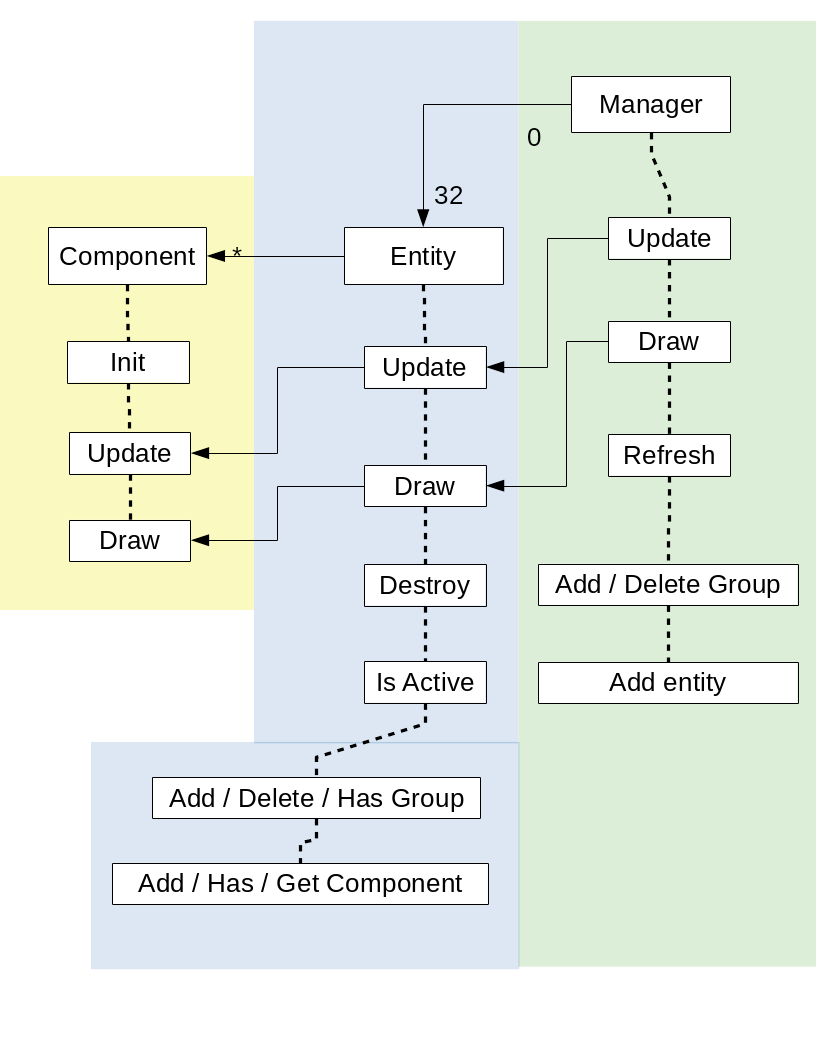
\includegraphics[scale=0.25]{Scheme}
  \caption{Entity-Component-System Verhältnisse}
  \label{fig:ECS}
\end{figure}

\end{document}
